\chapter{Solving DSGE models - basics} \label{ch:solbase}

This chapter covers everything that leads to, and stems from, the solution of DSGE models; a vast terrain. That is to say that the term ``solution'' in the title of the chapter is used rather broadly. You may be interested in simply finding the solution functions to a set of first order conditions stemming from your model, but you may also want to go a bit further. Typically, you may be interested in how this system behaves in response to shocks, whether temporary or permanent. Likewise, you may want to explore how the system comes back to its steady state or moves to a new one. This chapter covers all these topics. But instead of skipping to the topic closest to your needs, we recommend that you read this chapter chronologically, to learn basic Dynare commands and the process of writing a proper .mod file - this will serve as a base to carry out any of the above computations. 

\section{An important distinction}
Before speaking of Dynare, it is important recognize a distinction in model types. This distinction will appear throughout the chapter; in fact, it is so fundamental, that we considered writing separate chapters altogether. But the amount of common material - Dynare commands and syntax - is notable and writing two chapters would have been overly repetitive. Enough suspense; here is the important distinction: \textbf{is your model stochastic or deterministic?}\\

The distinction hinges on \textbf{whether future shocks are known}. In deterministic models, the occurrence of all future shocks is known exactly at the time of computing the model's solution. In stochastic models, instead, only the distribution of future shocks is known. Thus, deterministic models can be solved exactly. Stochastic models must be approximated. Intuitively, if an agent has perfect foresight, she can specify today what each of her precise actions will be in the future. But when the future has a random component to it, the best the agent can do is specify a decision rule for the future: what will her optimal action be contingent on each possible realization of a shock. It is therefore much harder to solve a stochastic model than a deterministic one: in the latter case we look for a series of numbers that match a set of given equations, whereas in the former, we search for a function which, to complicate things, may be non-linear and thus needs to be approximated. In control theory, the latter is usually called a ``closed loop'' solution, and the former an ``open loop''.\\

Because this distinction will resurface again and again throughout the chapter, but also because it has been a source of significant confusion in the past, the following gives some additional details. 

\subsection{\textsf{NOTE!} Deterministic vs stochastic models}

\textbf{Deterministic} models have the following characteristics:
\begin{enumerate}
\item As the DSGE (read, ``stochastic'', i.e. not deterministic!) literature has gained attention in economics, deterministic models have become somewhat rare. Examples include OLG models without aggregate uncertainty.
\item These models are usually introduced to study the impact of a change in regime, as in the introduction of a new tax, for instance. 
\item Models assume full information, perfect foresight and no uncertainty around shocks.
\item Shocks can hit the economy today or at any time in the future, in which case they would be expected with perfect foresight. They can also last one or several periods.
\item Most often, though, models introduce a positive shock today and zero shocks thereafter (with certainty).
\item The solution does not require linearization, in fact, it doesn't even really need a steady state. Instead, it involves numerical simulation to find the exact paths of endogenous variables that meet the model's first order conditions and shock structure. 
\item This solution method can therefore be useful when the economy is far away from steady state (when linearization offers a poor approximation).
\end{enumerate}
\textbf{Stochastic} models, instead, have the following characteristics:
\begin{enumerate}
\item These types of models tend to be more popular in the literature. Examples include most RBC models, or new keynesian monetary models.
\item In these models, shocks hit today (with a surprise), but thereafter their expected value is zero. Expected future shocks, or permanent changes in the exogenous variables cannot be handled due to the use of Taylor approximations around a steady state.
\item Note that when these models are linearized to the first order, agents behave as if future shocks where equal to zero (since their expectation is null), which is the \textbf{certainty equivalence property}. This is an often overlooked point in the literature which misleads readers in supposing their models may be deterministic.
\end{enumerate}


\section{Introducing an example}
The goal of this first section is to introduce a simple example. Future sections will aim to code this example into Dynare and analyze its salient features under the influence of shocks - both in a stochastic and a deterministic environment. Note that as a general rule, the examples in the basic chapters, \ref{ch:solbase} and \ref{ch:estbase}, are kept as bare as possible, with just enough features to help illustrate Dynare commands and functionalities. More complex examples are instead presented in the advanced chapters.\\

The model introduced here is a basic RBC model with monopolistic competition, used widely in the literature and taken, in its aspect presented below, from notes available on Jesus Fernandez-Villaverde's very instructive \href{http://www.econ.upenn.edu/~jesusfv/}{website}; this is a good place to look for additional information on any of the following model set-up and discussion.\\

Households maximize consumption, $c_t$ and leisure, $1-l_t$, where $l_t$ is labor input, according to the following utility function
\[
\mathbb{E}_t \sum_{t=0}^{\infty} \beta \left[ \log c_t + \psi \log(1-l_t) \right]
\]
and subject to the following budget constraint
\[
c_t + k_{t+1}=w_t l_t + r_t k_t + (1-\delta)k_t, \qquad \forall t>0
\]
where $k_t$ is capital stock, $w_t$ real wages, $r_t$ real interest rates or cost of capital and $\delta$ the depreciation rate. \\

The above equation can be seen as an accounting identity, with total expenditures on the left hand side and revenues - including the liquidation value of the capital stock - on the right hand side. Alternatively, with a little more imagination, the equation can also be interpreted as a capital accumulation equation after bringing $c_t$ to the right hand side and noticing that $w_t l_t + r_t k_t$, total payments to factors, equals $y_t$, or aggregate output, by the zero profit condition. As a consequence, if we define investment as $i_t=y_t - c_t$, we obtain the intuitive result that $i_t=k_{t+1} - (1-\delta) k_{t}$, or that investment replenishes the capital stock thereby countering the effects of depreciation. In any given period, the consumer therefore faces a tradeoff between consuming and investing in order to increase the capital stock and consuming more in following periods (as we will see later, production depends on capital).\\

Maximization of the household problem with respect to consumption, leisure and capital stock, yields the Euler equation in consumption, capturing the intertemporal tradeoff mentioned above, and the labor supply equation linking labor positively to wages and negatively to consumption (the wealthier, the more leisure due to the decreasing marginal utility of consumption). These equation are
\[
\frac{1}{c_t}=\beta \frac{1}{c_{t+1}} \left( 1 + r_{t+1} - \delta \right)
\]
and
\[
\psi \frac{c_t}{1-l_t}= w_t
\]

The firm side of the problem is slightly more involved, due to monopolistic competition, but is presented below in the simplest possible terms, with a little hand-waiving involved, as the derivations are relatively standard. \\

There are two ways to introduce monopolistic competition. We can either assume that firms sell differentiated varieties of a good to consumers who aggregate these according to a CES index. Or we can postulate that there is a continuum of intermediate producers with market power who each sell a different variety to a competitive final goods producer whose production function is a CES aggregate of intermediate varieties.\\

If we follow the second route, the final goods producer chooses his or her optimal demand for each variety, yielding the Dixit-Stiglitz downward sloping demand curve. Intermediate producers, instead, face a two pronged decision: how much labor and capital to employ given these factors' perfectly competitive prices and how to price the variety they produce.\\

Production of intermediate goods follows a CRS production function defined as
\[
y_{it} = k_{it}^\alpha (e^{z_t} l_{it})^{1-\alpha}
\]
where the $i$ subscript stands for firm $i$ of a continuum of firms between zero and one and where $\alpha$ is the capital elasticity in the production function, with $0<\alpha<1$. Also, $z_t$ captures technology which evolves according to
\[
z_t = \rho z_{t-1} + \epsilon_t
\]
where $\rho$ is a parameter capturing the persistence of technological progress and $\epsilon_t \thicksim \mathcal{N}(0,\sigma)$. \\

The solution to the sourcing problem yields an optimal capital to labor ratio, or relationship between payments to factors:
\[
k_{it}r_t=\frac{\alpha}{1-\alpha}w_tl_{it}
\]

The solution to the pricing problem, instead, yields the well-known constant markup pricing condition of monopolistic competition:
\[
p_{it}=\frac{\epsilon}{\epsilon -1}mc_t p_t
\]
where $p_{it}$ is firm $i$'s specific price, $mc_t$ is real marginal cost and $p_t$ is the aggregate CES price or average price. An additional step simplifies this expression: symmetric firms implies that all firms charge the same price and thus $p_{it}=p_t$; we therefore have: $mc_t = (\epsilon - 1)/\epsilon$ \\

But what are marginal costs equal to? To find the answer, we combine the optimal capital to labor ratio into the production function and take advantage of its CRS property to solve for the amount of labor or capital required to produce one unit of output. The real cost of using this amount of any one factor is given by $w_tl_{it} + r_tk_{it}$ where we substitute out the payments to the other factor using again the optimal capital to labor ratio. When solving for labor, for instance, we obtain
\[
mc_t = \left( \frac{1}{1-\alpha}�\right)^{1-\alpha} \left( \frac{1}{\alpha}�\right)^\alpha \frac{1}{A_t}w_t^{1-\alpha} r_t^\alpha
\]
which does not depend on $i$; it is thus the same for all firms. \\

Interestingly, the above can be worked out, by using the optimal capital to labor ratio, to yield $w_t [(1-\alpha)y_{it}/l_{it}]^{-1}$, or $w_t \frac{\partial l_{it}}{\partial y_{it}}$, which is the definition of marginal cost: the cost in terms of labor input of producing an additional unit of output. This should not be a surprise since the optimal capital to labor ratio follows from the maximization of the production function (minus real costs) with respect to its factors. \\

Combining this result for marginal cost, as well as its counterpart in terms of capital, with the optimal pricing condition yields the final two important equations of our model
\[
w_t = (1-\alpha) \frac{y_{it}}{l_{it}} \frac{(\epsilon-1)}{\epsilon}
\]
and
\[
r_t = \alpha \frac{y_{it}}{k_{it}} \frac{(\epsilon-1)}{\epsilon}
\]

To end, we aggregate the production of each individual firm to find an aggregate production function. On the supply side, we factor out the capital to labor ratio, $k_t/l_t$, which is the same for all firms and thus does not depend on $i$. On the other side, we have the Dixit-Stiglitz demand for each variety. By equating the two and integrating both side, and noting that price dispersion is null - or that, as hinted earlier, $p_{it}=p_t$ - we obtain aggregate production
\[
y_t = A_t k_t^\alpha l_t^{1-\alpha}
\]
which can be shown is equal to the aggregate amount of varieties bought by the final good producer (according to a CES aggregation index) and, in turn, equal to the aggregate output of final good, itself equal to household consumption. Note, to close, that because the ratio of output to each factor is the same for each intermediate firm and that firm specific as well as aggregate production is CRS, we can rewrite the above two equations for $w_t$ and $r_t$ without the $i$ subscripts on the right hand side. \\

This ends the exposition of the example. Now, let's roll up our sleeves and see how we can input the model into Dynare and actually test how the model will respond to shocks. 

\section{Dynare .mod file structure}
Input into Dynare involves the .mod file, as mentioned loosely in the introduction of this Guide. The .mod file can be written in any editor, external or internal to Matlab. It will then be read by Matlab by first navigating within Matlab to the directory where the .mod file is stored and then by typing in the Matlab command line \texttt{Dynare filename.mod;} (although actually typing the extension .mod is not necessary). But before we get into executing a .mod file, let's start by writing one! \\

It is convenient to think of the .mod file as containing four distinct blocks, illustrated in figure \ref{fig:modstruct}:
\begin{itemize}
\item \textbf{preamble}: lists variables and parameters
\item \textbf{model}: spells out the model
\item \textbf{transition}: gives indications to find the steady state and defines the shocks to the system
\item \textbf{computation}: instructs Dynare to undertake specific operations (e.g. forecasting, estimating impulse response functions)
\end{itemize}
Our exposition below will structured according to each of these blocks. 
\begin{figure} \label{fig:modstruct}
\begin{center} 
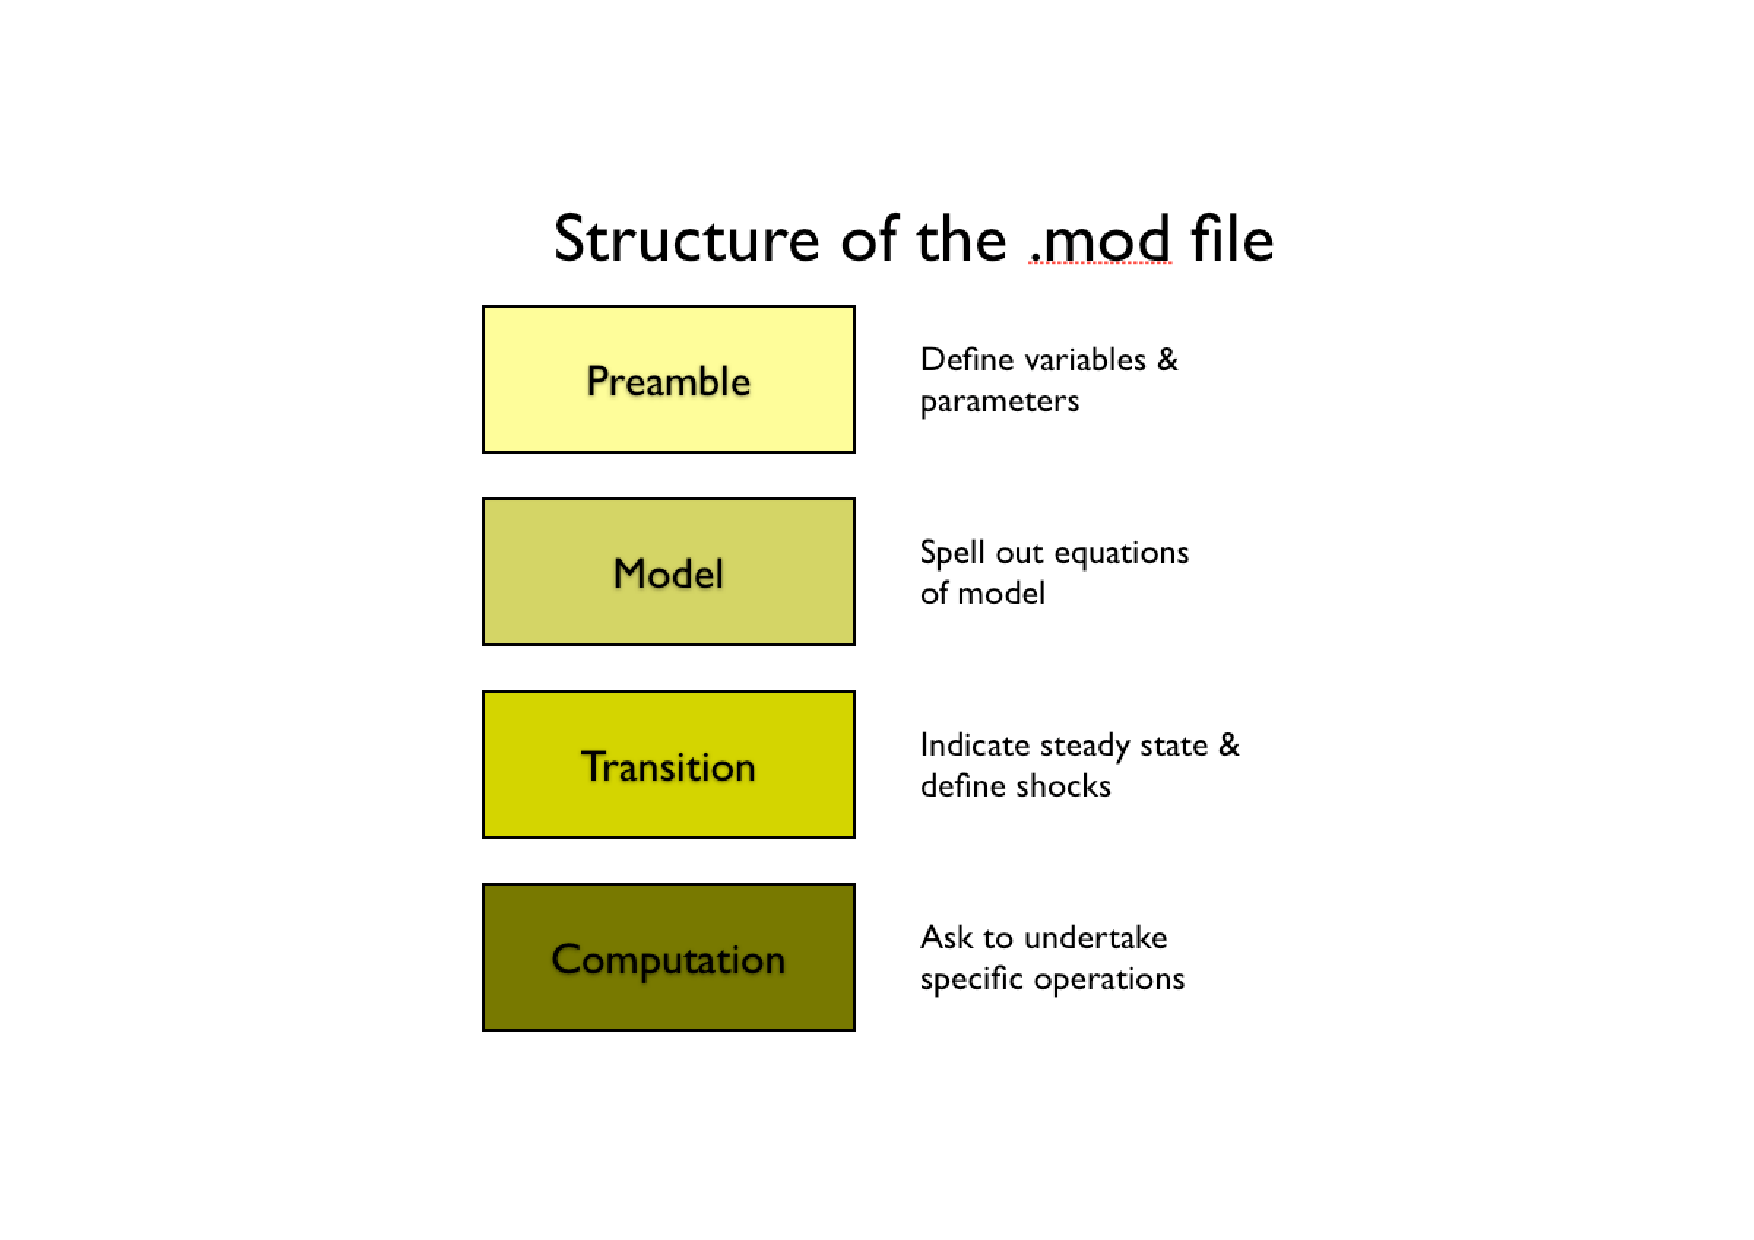
\includegraphics[width=1.0\textwidth]{P_ModStruct3} 
\end{center} 
\caption[Structure of the .mod file]{The .mod file contains four logically distinct parts.} 
\end{figure}

\section{Filling out the preamble}
The preamble generally involves three commands that tell Dynare what are the model's variables, which are endogenous and what are the parameters. The \textbf{commands} are:
\begin{itemize}
\item \texttt{var} starts the list of endogenous variables, to be separated by commas. 
\item \texttt{varexo} starts the list of exogenous variables that will be shocked.
\item \texttt{parameters} starts the list of parameters and assigns values to each.
\end{itemize}

In the case of our example, here's what the \textbf{preamble would look like}:\\ 
\\
\texttt{var y, c, k, a, h, b;\\
varexo e,u;\\
parameters beta, rho, beta, alpha, delta, theta, psi, tau;\\
alpha = 0.36;\\
rho   = 0.95;\\
tau   = 0.025;\\
beta  = 0.99;\\
delta = 0.025;\\
psi   = 0;\\
theta = 2.95;\\
phi   = 0.1;}\\

As you can tell, writing a .mod file is really quite straightforward. Two quick comments: \textsf{\textbf{TIP!}} Remember that each line of the .mod file must be terminated by a semicolon (;). To comment out any line, start the line with two forward slashes (//).  

\section{Specifying the model} \label{sec:modspe}
\subsection{Model in Dynare notation}
One of the beauties of Dynare is that you can input your model's equations almost as if you were writing them to communicate them to a person - not a machine. No fancy transformations, no matrix manipulations, no ambiguous deliberations about the backward or forward looking nature of variables are necessary. Dynare's pre-processor does all the grunt work to build and populate the various matrices necessary to untangle and solve the system. Let's first have a look at our model in Dynare notation, and then take a moment to point out some of its important features. \\
\\
\texttt{model;\\
c*theta*h$\hat{ }$(1+psi)=(1-alpha)*y;\\
k = beta*(((exp(b)*c)/(exp(b(+1))*c(+1)))\\
    *(exp(b(+1))*alpha*y(+1)+(1-delta)*k));\\
y = exp(a)*(k(-1)$\hat{ }$alpha)*(h$\hat{ }$(1-alpha));\\
k = exp(b)*(y-c)+(1-delta)*k(-1);\\
a = rho*a(-1)+tau*b(-1) + e;\\
b = tau*a(-1)+rho*b(-1) + u;\\
end;}\\

\subsection{Some commands and conventions}
The above example illustrates the use of a few important commands and conventions to translate a model into a Dynare-readable .mod file. 
\begin{itemize}
\item The first thing to notice, is that the model block of the .mod file begins with the command \texttt{model} and ends with the command \texttt{end}. 
\item Second, in between, there need to be as many equations as you declared endogenous parameters (this is actually one of the first things that Dynare checks; it will immediately let you know if there are any problems). 
\item Third, as in the preamble and everywhere along the .mod file, each line ends with a semicolon (except when a line is too long and you want to break it across two lines). 
\item Fourth, equations are entered one by one, with the same variable and parameter names as declared in the preamble. 
\item Fifth, the specification of the equations looks almost identical to those listed as the first order conditions above, except for a few important differences. These make up the variable input conventions and are listed in the box below for greater clarity.
\end{itemize}

\begin{tabular}{|p{11cm}|}
\hline
\textbf{Variable input conventions}\\
\begin{enumerate}
\item Variables entering the system with a time $t$ subscript are written plainly. For example, $x_t$ would be written $x$. 
\item Variables entering the system with a time $t-n$ subscript are written with $(-n)$ following them. For example, $x_{t-2}$ would be written $x(-2)$ (incidentally, this would count as two backward looking variables). 
\item In the same way, variables entering the system with a time $t+n$ subscript are written with $(+n)$ following them. For example, $x_{t+2}$ would be written $x(+2)$.
\item The only slight complications has to do with stock variables. One rule that may help is: in Dynare, the timing of each variable reflects when that variable is decided. For instance, our capital stock today is not decided today, but yesterday (recall, it is a function of yesterday's investment and capital stock). Thus, we would write it with a lag, meaning that the $k_{t+1}$ in our model equations gets reported into the .mod file as $k$ (at time $t$).
\item A slightly more roundabout way to explain the same thing is that for stock variables, you must use a ``stock at the end of the period'' concept. It is investment during period $t$ that sets stock at the end of period $t$. Be careful, a lot of papers use the ``stock at the beginning of the period'' convention. For instance, in some wage negociation models, wages used during a period are set the period before. In the equation for wages, you can write wage in period $t$ (when they are set), but in the labor demand equation, wages should appear with a one period lag. 
\end{enumerate}
\\
\hline
\end{tabular}\\
\\

\subsection{Predetermined vs. non-predetermined variables}
What does all this mean for predetermined vs. non-predetermined variables? If you are used to solving simple DSGE models by hand, or to inputting the matrices corresponding to your equations, you are probably eagerly waiting for an answer. \textsf{\textbf{TIP!}} Actually, you may surprised (relieved?!) to know that Dynare figures out automatically which variables are predetermined and non-predetermined. Especially in more complicated models, the categorization of variables can be difficult, if not ambiguous, and a source of much frustration.\\ 

In Dynare, a forward-looking variable is a variable that appears in the model with a lead. For example, $c(+1)$.  A predetermined variable is a variable that appears with a lag. Note that a variable can be both forward-looking and predetermined. A static variable is a variable that appears in the model with neither a lead or a lag.\\

\subsection{Linear and log-linearized models}
There are two other variants of the system's equations which Dynare accommodates. First, the \textbf{linear model} and second, the \textbf{model in exp-logs}. In the first case, all that is necessary is to write the term \texttt{(linear)} next to the command \texttt{model}. In our example, this would yield the following for the first two lines:\\

** complete once the fixed problem with linearized equations\\

Otherwise, you may be interested to have Dynare take Taylor series expansions in logs rather than in levels. If so, simply rewrite your equations by taking $\exp$ and $\log$ of each variable. The Dynare input convention makes this very easy to do. Our example would need to be re-written as:\\
\\
\texttt{model;\\
exp(c)*theta*exp(h)$\hat{ }$(1+psi)=(1-alpha)*exp(y);\\
exp(k) = beta*(((exp(b)*exp(c))/(exp(b(+1))*exp(c(+1))))\\
         *(exp(b(+1))*alpha*exp(y(+1))+(1-delta)*exp(k)));\\
exp(y) = exp(a)*(exp(k(-1))$\hat{ }$alpha)*(exp(h)$\hat{ }$(1-alpha));\\
exp(k) = exp(b)*(exp(y)-exp(c))+(1-delta)*exp(k(-1));\\
a = rho*a(-1)+tau*b(-1) + e;\\
b = tau*a(-1)+rho*b(-1) + u;\\
end;}\\
so that the levels of variables are given by $\exp(variable)$.\\

\subsection{Taking advantage of Matlab}
(\textbf{\textsf{TIP!}}) Dynare accepts standard Matlab expressions in any of the model equations. The only thing you need to do is to start the line with \# and then enter the Matlab command as you would normally. For example, if you want to define a variable in terms of another, you can write \texttt{\# b = 1 / c}. This feature, actually, is more useful when carrying out model estimation and wanting to declare transformations of parameters. 

\section{Specifying dynamics (steady states and shocks)}
In the ``dynamics'' block of the .mod file, you need to specify two things: steady state values and shocks to the exogenous variables; basically, where is your model starting from (steady state, usually) and where is it going (due to the shocks)? Let's briefly describe the relevant commands and then worry about how to mix and match them depending on the type of shock you want to create and the type of model you're dealing with.\\

\subsection{Specifying steady states}
To specify steady states, you use the commands \texttt{initval}, \texttt{endval} or, more rarely, \texttt{histval}. Each command initiates a block which must be terminated by \texttt{end}. In the middle, you should list values for all your variables - endogenous and exogenous (even if the latter is not required for stochastic models, but you may want to get in the habit of doing so anyhow). The \texttt{initval} command allows you to enter your variables' steady state values before any shocks hit the system. Under the \texttt{endval} command, instead, you would list the steady state values to which the system moves after any shocks (assuming the system does not return to its original steady state). Finally, the \texttt{histval} command allows you to specify different historical initial values for different periods, in case you have lagged variables. But because this last command is rarely used, we will not dwell on it; you can instead read more about it in the Reference Manual (** add link). We now focus on the \texttt{intival} block, which is common to all .mod files, and then return later to the \texttt{endval} block, which should be used only in certain circumstances. \\

For our example, here is what the \texttt{initval} block would look like:\\
\\
\texttt{initval;\\
y = 1.08068253095672;\\
c = 0.80359242014163;\\
h = 0.29175631001732;\\
k = 5;\\
a = 0;\\
b = 0;\\
e = 0;\\
u = 0;\\
end;}\\

The difficulty here, of course, is calculating the actual steady state values. Because this is such a central topic, although it borders on a form of art, rather than a science, we've devoted the box below to some \textsf{\textbf{TIPS!}} regarding the calculation of steady states.\\

\begin{tabular}{|p{11cm}|}
\hline
\textbf{Calculating steady states}\\
\\
Suppose, first, that you were interested in entering the exact values of your model's steady states. You could, most straightforwardly, use an external program to calculate these values, like Maple and then enter them by hand. But of course, this procedure could be time consuming and bothersome, especially if you want to alter parameter values. \\

Actually, Dynare can take care of finding your model's steady state by calling the appropriate Matlab functions. To do so, you still need to provide an initial guess of your steady state in the \texttt{initval} block, but you would follow the block with the command \texttt{steady[ \textsl{option} ]}. This will instruct Matlab to use an iterative procedure to find the model's steady state. The procedure itself depends on the option you specify. Possible options are:\texttt{solve\_algo = 0}: uses Matlab Optimization Toolbox FSOLVE; \texttt{solve\_algo = 1}: uses Dynare�s own nonlinear equation solver; and \texttt{solve\_algo = 2}: splits the model into recursive blocks and solves each block in turn. The latter is the default option if none is specified. \\

For complicated models, finding good numerical initial values for the endogenous variables is the trickiest part of finding the equilibrium of that model. Often, it is better to start with a smaller model and add new variables one by one.\\

Unfortunately, for simpler models, you may still run into difficulties in finding your steady state. If so, one option is still available: that of entering your model in linear terms (where variables are expressed in percent deviations from steady state) and thus specifying your steady state values in the \texttt{initval} block as all being zero. \\
\\
\hline
\end{tabular}\\
\\

** USED TO BE DET STOCH DIFFERENCE*** \\

\subsection{Adding shocks}
Now let's see how this section's relevant commands - specifying initial and final values, as well as shocks - all fit together depending on the type of model you are using. Figure \ref{fig:shockmodel} summarizes the possible combinations of commands and their usefulness. 
\begin{figure} \label{fig:shockmodel}
\begin{center} 
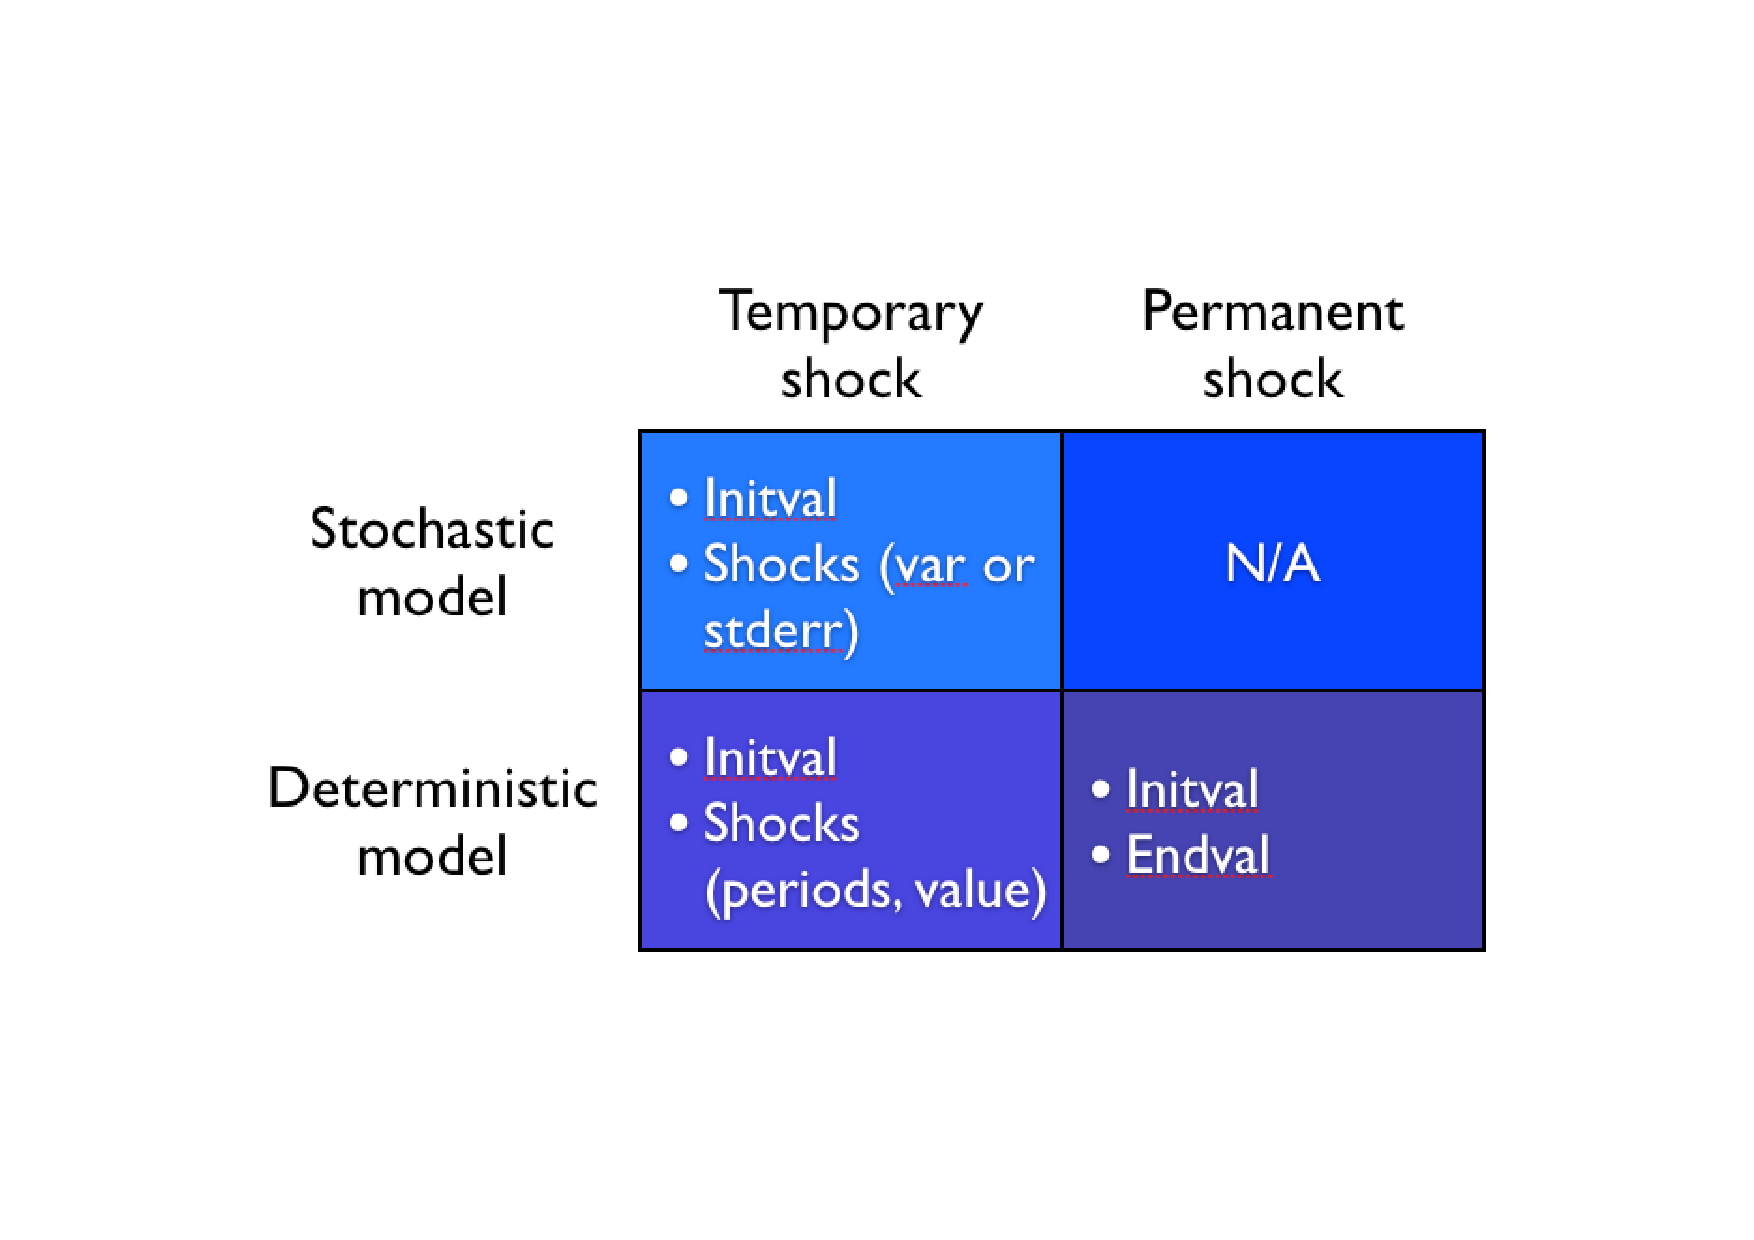
\includegraphics[width=1.0\textwidth]{P_ShockModel2} 
\end{center} 
\caption[Shock and model-type matrix]{Depending on the model type you're working with and the desired shocks, you will need to mix and match the various steady state and shock commands.} 
\end{figure}\\

As seen in the figure, when working with a deterministic model, you have the choice of introducing both temporary and permanent shocks. In the \textbf{deterministic-temporary} case, you are free to set the duration and level of the shock. To specify a shock that lasts 9 periods on $\epsilon_t$, for instance, you would write (** is this a 10\% shock?)\\
\\
\texttt{shocks;\\
var e;
periods 1:9;\\
values 0.1;\\
end;}\\

In the \textbf{deterministic-permanent} case, you would not specify actual ``shocks'', but would simply tell the system to which steady state values you would like it to move to and let Dynare calculate the transition path. To do so, you would use the \texttt{endval} block following the usual \texttt{initval} block. For instance, you may specify all values to remain common between the two blocks, except for the value of the exogenous variable that changes permanently. The example we have used so far is somewhat ill-suited to illustrate this sort of permanent change, since if the exogenous shocks were positive always, they would make the technology variables $a_t$ and $b_t$ explode. Thus, for illustrative purposes, we could imagine getting rid of the last two equations of our system (the equations of motion of the technology variables) as well as the variables $\epsilon_t$ and $\nu_t$, and simply making $a_t$ and $b_t$ exogenous. In that case, we could use the following blocks in our .mod file to introduce a permanent increase in productivity: \\
\\
\texttt{initval;\\
y = 1.08068253095672;\\
c = 0.80359242014163;\\
h = 0.29175631001732;\\
k = 5;\\
a = 0;\\
b = 0;\\
end;\\
\\
endval;\\
y = 1.08068253095672;\\
c = 0.80359242014163;\\
h = 0.29175631001732;\\
k = 5;\\
a = 0.1;\\
b = 0;\\
end;\\
\\
steady;}\\
\\
where the last command \texttt{steady} was added since the \texttt{endval} values are bound to be somewhat imprecise now that we have changed the value of $a_t$. \\

In case of a \textbf{stochastic-temporary} model, which is really what makes most sense for the example introduced earlier, we can only specify a temporary shock lasting one period. In the case of our example, we would write:\\
\\
\texttt{shocks;\\
var e; stderr 0.009;\\
var u; stderr 0.009;\\
var e, u = phi*0.009*0.009;\\
end;}\\
\\
where the last line specifies the contemporaneous correlation between our two exogenous variables. Note that to introduce the variance of the shock, we could also have written: (** does this mean every time you run your .mod file you will get a slightly different shock?)\\
\\
\texttt{shocks;\\
var e = 0.009 $\hat{}$ 2;\\
var u = 0.009 $\hat{}$ 2;\\
var e, u = phi*0.009*0.009;\\
end;}\\

\subsection{Some useful details}
Two last things to note: first, you can actually \textbf{mix in deterministic shocks} in stochastic models by using the commands \texttt{varexo\_det} and listing some shocks as lasting more than one period in the \texttt{shocks} block. For information on how to do so, please see the Reference Manual (** add link).\\

Second, a handy command that you can add after the \texttt{initval} or \texttt{endval} block (following the \texttt{steady} command if you decide to add on) is the \texttt{check} command. This computes and displays the eigenvalues of your system which are used in the solution method. A necessary condition for the uniqueness of a stable equilibrium in the neighborhood of the steady state is that there are 
as many eigenvalues larger than one in modulus as there are forward looking variables in the system. If this condition is not met, Dynare will tell you that the Blanchard-Kahn conditions are not satisfied (whether or not you insert the \texttt{check} command). \\

One thing to note: don't worry if you get infinite eigenvalues - these are are firmly grounded in the theory of generalized eigenvalues. They have no detrimental influence on the solution algorithm. As far as Blanchard-Kahn conditions are concerned infinite eigenvalues counted as explosive roots of modulus larger than one. \\

\subsection{The complete dynamics of the .mod file}
Let's bring together all the disparate parts discussed above in order to get a complete view of what the "dynamics" part of the .mod file looks like for our ``stochastic-temporary shock'' type model (we've seen only bits and pieces of it so far...).\\
\\
\texttt{initval;\\
y = 1.08068253095672;\\
c = 0.80359242014163;\\
h = 0.29175631001732;\\
k = 5;\\
a = 0;\\
b = 0;\\
e = 0;\\
u = 0;\\
end;\\
\\
shocks;\\
var e; stderr 0.009;\\
var u; stderr 0.009;\\
var e, u = phi*0.009*0.009;\\
end;}\\

\section{Selecting a computation} \label{sec:compute}
So far, we have written an instructive .mod file, but what should Dynare do with it? What are we interested in? In most cases, it will be impulse response functions (IRFs) due to the external shocks. Let's see which are the appropriate commands to give to Dynare.\\

\subsection{For deterministic models}
In the deterministic case, all you need to do is add the command \texttt{simul} at the bottom of your .mod file. Note that the command takes the option \texttt{[ (periods=INTEGER) ] }. \texttt{Simul} triggers the computation of a deterministic simulation of the model for the number of periods set in the option. To do so, it uses a Newton method to solve simultaneously all the equations for every period (see \citet{Juillard1996} for details). \textbf{The simulated variables} are available in global matrix y\_ in which variables are arranged row by row, in alphabetical order. \\

\subsection{For stochastic models}
In the more popular case of a stochastic model, as in our example, the command \texttt{stoch\_simul} is appropriate. This command instructs Dynare to compute a Taylor approximation of the decision and transition functions for the model (the equations listing current values of the endogenous variables of the model as a function of the previous state of the model and current shocks), impulse response 
functions and various descriptive statistics (moments, variance decomposition, correlation and autocorrelation coeffi- 
cients).\footnote{For correlated shocks, the variance decomposition is computed as in the VAR literature through a Cholesky 
decomposition of the covariance matrix of the exogenous variables. When the shocks are correlated, the variance 
decomposition depends upon the order of the variables in the varexo command. (** not sure I understand this).} If you're interested to peer a little further into what exactly is going on behind the scenes of Dynare's computations, have a look at Chapter \ref{ch:soladv}. Here instead, we focus on the application of the command and reproduce below the table of options that can be added to \texttt{stoch\_simul}. (** maybe just include a subset and refer to Ref Man for complete set?) \\

\textbf{Options following the \texttt{stoch\_simul} command:}\\
\begin{itemize}
\item ar = INTEGER: Order of autocorrelation coefficients to compute and to print (default = 5).
\item dr\_algo = 0 or 1: specifies the algorithm used for computing the quadratic approximation of the decision rules: $0$ uses a pure perturbation approach as in \citet{SchmittGrohe2004} (default) and 1 moves the point around which the Taylor expansion is computed toward the means of the distribution as in \citet{CollardJuillard2001a}.
\item drop = INTEGER: number of points dropped at the beginning of simulation before computing the summary 
statistics (default = 100).
\item hp\_filter = INTEGER: uses HP filter with lambda = INTEGER before computing moments (default: no filter).
\item hp\_ngrid = INTEGER: number of points in the grid for the discreet Inverse Fast Fourier Transform used in the 
HP filter computation. It may be necessary to increase it for highly autocorrelated processes (default = 512).
\item irf = INTEGER: number of periods on which to compute the IRFs (default = 40). Setting IRF=0, suppresses the 
plotting of IRF�s. 
\item relative\_irf requests the computation of normalized IRFs in percentage of the standard error of each shock.
\item nocorr: doesn�t print the correlation matrix (printing is the default).
\item nofunctions: doesn�t print the coefficients of the approximated solution (printing is the default). 
\item nomoments: doesn�t print moments of the endogenous variables (printing them is the default).
\item noprint: cancel any printing; usefull for loops. 
\item order = 1 or 2 : order of Taylor approximation (default = 2), unless you're working with a linear model in which case the order is automatically set to 1.  
\item periods = INTEGER: specifies the number of periods to use in simulations (default = 0). 
\item qz\_criterium = INTEGER or DOUBLE: value used to split stable from unstable eigenvalues in reordering the 
Generalized Schur decomposition used for solving 1st order problems (default = 1.000001).
\item replic = INTEGER: number of simulated series used to compute the IRFs (default = 1 if order = 1, and 50 
otherwise).
\item simul\_seed = INTEGER or DOUBLE or (EXPRESSION): specifies a seed for the random generator so as to obtain the 
same random sample at each run of the program. Otherwise a different sample is used for each run (default: seed 
not specified). (** not sure I understand this)
\end{itemize}

Going back to our good old example, suppose we are interested in printing all the various measures of moments of our variables, want to see impulse response functions for all variables, are basically happy with all default options and want to carry out simulations over a good number of periods. We would then end our .mod file with the following command:\\
\\
\texttt{stoch\_simul(periods=2100);}\\

\section{The complete .mod file}
For completion's sake, and for the pleasure of seeing our work bear its fruits, here is the complete .mod file corresponding to our example:\\
\\
\texttt{var y, c, k, a, h, b;\\
varexo e,u;\\
parameters beta, rho, beta, alpha, delta, theta, psi, tau;\\
alpha = 0.36;\\
rho   = 0.95;\\
tau   = 0.025;\\
beta  = 0.99;\\
delta = 0.025;\\
psi   = 0;\\
theta = 2.95;\\
phi   = 0.1;\\
\\
model;\\
c*theta*h$\hat{ }$(1+psi)=(1-alpha)*y;\\
k = beta*(((exp(b)*c)/(exp(b(+1))*c(+1)))\\
    *(exp(b(+1))*alpha*y(+1)+(1-delta)*k));\\
y = exp(a)*(k(-1)$\hat{ }$alpha)*(h$\hat{ }$(1-alpha));\\
k = exp(b)*(y-c)+(1-delta)*k(-1);\\
a = rho*a(-1)+tau*b(-1) + e;\\
b = tau*a(-1)+rho*b(-1) + u;\\
end;\\
\\
initval;\\
y = 1.08068253095672;\\
c = 0.80359242014163;\\
h = 0.29175631001732;\\
k = 5;\\
a = 0;\\
b = 0;\\
e = 0;\\
u = 0;\\
end;\\
\\
shocks;\\
var e; stderr 0.009;\\
var u; stderr 0.009;\\
var e, u = phi*0.009*0.009;\\
end;\\
\\
stoch\_simul(periods=2100);}\\

As per our earlier discussion, we could have added \texttt{steady;} and \texttt{check;} after the \texttt{initval\ldots end;} block.

\section{Executing the .mod file and interpreting results}
To see this all come to life, run this .mod file, which is conveniently installed by default in the Dynare ``examples'' directory (the .mod file is called example1.mod). To run a .mod file, navigate within Matlab to the directory where the example1.mod is stored. You can do this by clicking in the ``current directory'' window of Matlab, or typing the path directly in the top white field of Matlab. Once there, all you need to do is place your cursor in the Matlab command window and type \texttt{dynare example1;} to execute your .mod file. \\

Running example1.mod should take at most 30 seconds. As a result, you should get two forms of output - tabular in the Matlab command window and graphical in two pop-up windows. The tabular results can be summarized as follows:
\begin{enumerate}
\item \textbf{Model summary:} a count of the various variable types in your model (endogenous, jumpers, etc...).
\item \textbf{Matrix of covariance of exogenous shocks:} this should square with the values of the shock variances and co-variances you provided in the .mod file.
\item \textbf{Policy and transition functions:} Solving the rational exectation model, $\mathbb{E}_t[f(y_{t+1},y_t,y_{t-1},u_t)]=0$ , means finding an unkown function, $y_t = g(y_{t-1},u_t)$  that could be plugged into the original model and satisfy the implied restrictions (the first order conditions). A first order approximation of this function can be written as $y_t = \bar{y} + g_y \hat{y}_{t-1} + g_u u_t$, with $\hat{y}_t = y_t-\bar{y}$ and $\bar{y}$ being the steadystate value of $y$, and where $g_x$ is the partial derivative of the $g$ function with respect to variable $x$. In other words, the function $g$ is a time recursive (approximated) representation of the model that can generate timeseries that will approximatively satisfy the rational expectation hypothesis contained in the original model. In Dynare, the table ``Policy and Transition function'' contains the elements of $g_y$ and $g_u$. Details on the policy and transition function can be found in Chapter \ref{ch:estadv}.
\item \textbf{Moments of simulated variables:} up to the fourth moments.
\item \textbf{Correlation of simulated variables:} these are the contemporaneous correlations, presented in a table.
\item \textbf{Autocorrelation of simulated variables:} up to the fifth lag, as specified in the options of \texttt{stoch\_simul}. 
\end{enumerate}

** Add graphical results (last minute omission, my mistake...)









